\documentclass[11pt,a4paper]{article}

% ------------------------------------------------------------------------------
% PACKAGES AND STYLING
% ------------------------------------------------------------------------------
\usepackage[utf8]{inputenc}
\usepackage[margin=1in]{geometry}
\usepackage{amsmath,amssymb,amsfonts}
\usepackage{graphicx}
\usepackage{booktabs}
\usepackage{tabularx}
\usepackage{array}
\usepackage{xcolor}
\usepackage{tikz}
\usetikzlibrary{arrows.meta,positioning,shapes.geometric,shapes.misc,calc,patterns}
\usepackage{listings}
\usepackage{fancyhdr}
\usepackage{cite}
\usepackage{microtype}
\usepackage[colorlinks=true,linkcolor=blue!70!black,citecolor=blue!70!black,urlcolor=blue!70!black]{hyperref}

% Page Header and Footer
\pagestyle{fancy}
\fancyhf{}
\rhead{\small\textit{KTP Technical Project Report}}
\cfoot{\thepage}

% Color definitions
\definecolor{primaryblue}{RGB}{37,99,235}
\definecolor{darkslate}{RGB}{30,41,59}
\definecolor{lightgray}{RGB}{248,250,252}
\definecolor{bordergray}{RGB}{203,213,225}
\definecolor{amber}{RGB}{245,158,11}
\definecolor{slate}{RGB}{100,116,139}

% Listing setup for C code snippets
\lstset{
  language=C,
  basicstyle=\ttfamily\small,
  keywordstyle=\color{primaryblue}\bfseries,
  commentstyle=\color{gray}\textit,
  stringstyle=\color{teal},
  numbers=left,
  numberstyle=\tiny\color{gray},
  stepnumber=1,
  numbersep=8pt,
  backgroundcolor=\color{lightgray},
  frame=single,
  rulecolor=\color{bordergray},
  tabsize=2,
  breaklines=true,
  breakatwhitespace=false,
  showspaces=false,
  showstringspaces=false
}

% ------------------------------------------------------------------------------
% TITLE AND METADATA
% ------------------------------------------------------------------------------
\title{
  \vspace{-1.5cm}
  \textbf{\Large Design, Implementation, and Empirical Evaluation of a User-Space Reliable Transport Protocol (KTP) over Unreliable Datagram Channels}
  \vspace{0.4cm}
}

\author{
  \textbf{Arpit Kumar} \\
  Indian Institute of Technology Kharagpur \\
  \texttt{Kharagpur, West Bengal, India}
}

\date{
  \today
}

% ------------------------------------------------------------------------------
% DOCUMENT BODY
% ------------------------------------------------------------------------------
\begin{document}

\maketitle

\begin{abstract}
Transport layer communication over packet-switched networks traditionally presents a dichotomy between the stream-oriented, connection-stateful reliability of TCP and the lightweight, message-oriented, yet unreliable datagram semantics of UDP. In specialized distributed systems, telecommand channels, and high-throughput transaction pipelines, applications require message-oriented atomicity coupled with deterministic, in-order, guaranteed delivery. This paper presents the design, formalization, implementation, and performance evaluation of the \textbf{KGP Transport Protocol (KTP)}, a user-space reliable transport subsystem implemented on top of raw POSIX UDP datagram sockets. 

KTP employs a decoupled multi-process architecture utilizing System V Shared Memory for socket abstraction and zero-copy queuing. A background protocol daemon hosts dual asynchronous worker threads: Thread $R$ conducts non-blocking I/O multiplexing via \texttt{select()} to handle incoming datagrams and ACK demultiplexing, while Thread $S$ manages monotonic timestamp timers and timeout-driven Automatic Repeat reQuest (ARQ) retransmissions. The protocol specifies a compact 3-byte wire header supporting up to 512-byte atomic payloads, sequence tracking modulo 256, and circular FIFO buffer management with strict boundary invariants. We provide comprehensive sequence traces for nominal handshakes, forward channel drop recovery, and reverse acknowledgment loss with receiver-side deduplication. Finally, empirical evaluations under synthetic packet drop probabilities ($p \in [0.05, 0.50]$) demonstrate robust convergence with transmission overhead tightly bounded between single-link and bidirectional geometric loss models.
\end{abstract}

\vspace{0.2cm}
\noindent\textbf{Keywords:} Transport Protocols, Reliable Data Transfer, ARQ, Shared Memory IPC, POSIX Multithreading, Flow Control, Packet Deduplication.

\section{Introduction}
\label{sec:introduction}

The transport layer of the Internet protocol suite serves as the operational bridge between host-to-host network routing and application-level inter-process communication. Under the classical End-to-End Argument articulated by Saltzer, Reed, and Clark~\cite{saltzer1984end}, end-to-end reliability, integrity, and duplicate suppression must ultimately reside within the endpoints rather than intermediate network nodes. 

In standard network programming, developers are typically confined to two standard transport layer primitives:
\begin{enumerate}
    \item \textbf{Transmission Control Protocol (TCP)}: A connection-oriented protocol providing full-duplex, ordered byte-stream delivery with congestion and flow control. However, TCP enforces continuous byte streams without inherent message boundary preservation, necessitating application-level framing or length-prefix parsing.
    \item \textbf{User Datagram Protocol (UDP)}: A connectionless, lightweight datagram service that preserves message boundaries atomically. However, UDP provides no guarantees regarding packet loss, ordering, duplication, or channel delay variations.
\end{enumerate}

To bridge this operational divide, the \textbf{KGP Transport Protocol (KTP)} was conceived as an extensible, user-space, message-oriented transport protocol. Rather than operating inside the Linux kernel, KTP implements transport abstractions entirely within user space via a shared library (\texttt{libksocket.a}) interfacing with a centralized background protocol daemon process (\texttt{ktp\_main}) through POSIX/System V shared memory.

The contributions of this work are summarized as follows:
\begin{itemize}
    \item \textbf{Multi-Process IPC Architecture}: A scalable shared-memory transport control structure maintaining multiple active socket descriptors across independent application processes.
    \item \textbf{Dual-Threaded Protocol Engine}: Decoupling the transmission and reception lifecycles into a non-blocking receiver thread (Thread $R$) using I/O multiplexing and a periodic sender/timer thread (Thread $S$).
    \item \textbf{Stop-and-Wait ARQ with Deduplication}: A robust timeout retransmission engine capable of recovering from forward packet loss and reverse acknowledgment loss while preventing buffer corruption.
    \item \textbf{Empirical Loss Evaluation}: Statistical validation of protocol recovery efficiency across synthetic loss rates $p \in [0.05, 0.50]$.
\end{itemize}

% ------------------------------------------------------------------------------
\section{Protocol Architecture and IPC Model}
\label{sec:architecture}

\subsection{System Decomposition}
KTP enforces a strict separation between user-space application logic and low-level protocol orchestration. A typical deployment consists of three distinct layers, as conceptualized in Figure~\ref{fig:architecture}:
\begin{enumerate}
    \item \textbf{Application Space}: Autonomous client and server programs (such as \texttt{user1.c} and \texttt{user2.c}) invoking KTP library primitives (\texttt{k\_socket}, \texttt{k\_bind}, \texttt{k\_sendto}, \texttt{k\_recvfrom}, \texttt{k\_close}).
    \item \textbf{Inter-Process Shared Memory}: A central System V shared memory segment identified by an IPC key generated via \texttt{ftok("/", 'a')}. This memory region holds an array of socket control blocks (\texttt{struct k\_sock}) shared concurrently across user applications and the daemon.
    \item \textbf{Protocol Daemon Engine}: A persistent background process (\texttt{ktp\_main.c}) hosting two POSIX worker threads ($S$ and $R$) responsible for network-level packet transmission, timer surveillance, and packet demultiplexing.
\end{enumerate}

\begin{figure}[htbp]
\centering
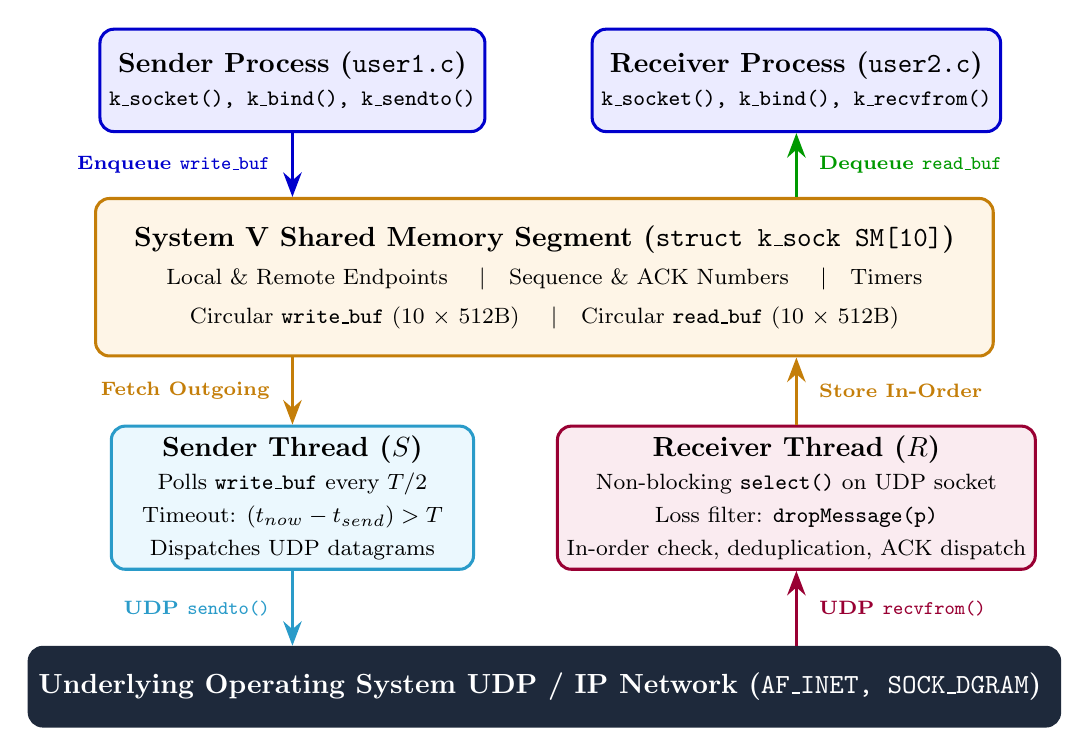
\begin{tikzpicture}[
  box/.style={draw=darkslate, rounded corners=5pt, line width=1.1pt, align=center, fill=white},
  appbox/.style={box, fill=blue!8, draw=blue!80!black, minimum width=4.6cm, minimum height=1.3cm},
  shmbox/.style={box, fill=amber!10, draw=amber!80!black, minimum width=11.4cm, minimum height=2.0cm},
  daemonbox/.style={box, fill=slate!8, draw=darkslate, minimum width=4.6cm, minimum height=1.6cm},
  netbox/.style={box, fill=darkslate, text=white, minimum width=11.4cm, minimum height=1.0cm},
  arrow/.style={-Stealth, line width=1.3pt}
]

  % Layer 1: Applications (Explicit horizontal positioning at -3.2 and +3.2)
  \node[appbox] (user1) at (-3.2, 2.5) {
    \textbf{Sender Process (\texttt{user1.c})} \\
    \footnotesize \texttt{k\_socket(), k\_bind(), k\_sendto()}
  };
  \node[appbox] (user2) at (3.2, 2.5) {
    \textbf{Receiver Process (\texttt{user2.c})} \\
    \footnotesize \texttt{k\_socket(), k\_bind(), k\_recvfrom()}
  };

  % Layer 2: Shared Memory (Centered at origin)
  \node[shmbox] (shm) at (0, 0) {
    \textbf{System V Shared Memory Segment (\texttt{struct k\_sock SM[10]})} \\[2pt]
    \footnotesize Local \& Remote Endpoints \quad$|$\quad Sequence \& ACK Numbers \quad$|$\quad Timers \\[2pt]
    \footnotesize Circular \texttt{write\_buf} (10 $\times$ 512B) \quad$|$\quad Circular \texttt{read\_buf} (10 $\times$ 512B)
  };

  % Layer 3: Daemon Threads (Explicit horizontal positioning at -3.2 and +3.2)
  \node[daemonbox, fill=cyan!8, draw=cyan!80!black] (threadS) at (-3.2, -2.8) {
    \textbf{Sender Thread ($S$)} \\
    \footnotesize Polls \texttt{write\_buf} every $T/2$ \\
    \footnotesize Timeout: $(t_{now} - t_{send}) > T$ \\
    \footnotesize Dispatches UDP datagrams
  };
  
  \node[daemonbox, fill=purple!8, draw=purple!80!black] (threadR) at (3.2, -2.8) {
    \textbf{Receiver Thread ($R$)} \\
    \footnotesize Non-blocking \texttt{select()} on UDP socket \\
    \footnotesize Loss filter: \texttt{dropMessage(p)} \\
    \footnotesize In-order check, deduplication, ACK dispatch
  };

  % Layer 4: Physical / OS Transport Network
  \node[netbox] (net) at (0, -5.2) {
    \textbf{Underlying Operating System UDP / IP Network (\texttt{AF\_INET, SOCK\_DGRAM})}
  };

  % Straight Vertical Connecting Lines with Outer-Margin Labels
  % user1 to SHM
  \draw[arrow, blue!80!black] (user1.south) -- node[left=0.15cm, font=\scriptsize\bfseries, text=blue!80!black] {Enqueue \texttt{write\_buf}} (user1.south |- shm.north);
  
  % SHM to user2
  \draw[arrow, green!60!black] (user2.south |- shm.north) -- node[right=0.15cm, font=\scriptsize\bfseries, text=green!60!black] {Dequeue \texttt{read\_buf}} (user2.south);

  % SHM to Thread S
  \draw[arrow, amber!80!black] (shm.south -| threadS.north) -- node[left=0.15cm, font=\scriptsize\bfseries, text=amber!80!black] {Fetch Outgoing} (threadS.north);
  
  % Thread R to SHM
  \draw[arrow, amber!80!black] (threadR.north) -- node[right=0.15cm, font=\scriptsize\bfseries, text=amber!80!black] {Store In-Order} (shm.south -| threadR.north);

  % Thread S to Net
  \draw[arrow, cyan!80!black] (threadS.south) -- node[left=0.15cm, font=\scriptsize\bfseries, text=cyan!80!black] {UDP \texttt{sendto()}} (threadS.south |- net.north);
  
  % Net to Thread R
  \draw[arrow, purple!80!black] (net.north -| threadR.south) -- node[right=0.15cm, font=\scriptsize\bfseries, text=purple!80!black] {UDP \texttt{recvfrom()}} (threadR.south);

\end{tikzpicture}
\caption{Architectural decomposition and inter-process communication topology of KTP.}
\label{fig:architecture}
\end{figure}

\subsection{Socket Control Block (\texttt{k\_sock})}
Each active KTP socket is represented inside shared memory by a dedicated control block. The structure definition in \texttt{ktp.h} is defined as follows:

\begin{lstlisting}[caption={KTP Socket Control Block Definition}]
typedef struct k_sock {
    int fd;                     // Underlying UDP socket file descriptor
    uint16_t dest_port;         // Peer UDP port in network byte order
    uint32_t dest_ip;           // Peer IPv4 address in network byte order
    uint16_t src_port;          // Local bound UDP port
    uint32_t src_ip;            // Local bound IPv4 address
    uint8_t seq_no;             // Sequence counter for outgoing packets
    uint8_t ack_no;             // Sequence counter expected from incoming packets
    uint8_t state;              // State: WAITING_FOR_DATA (0) or WAITING_FOR_ACK (1)
    queue read_buf;             // Circular buffer for delivered received payloads
    queue write_buf;            // Circular buffer for outgoing buffered payloads
    struct timespec send_time;  // Monotonic timestamp of last packet transmission
} k_sock;
\end{lstlisting}

Shared memory is configured to host an array of size $\text{SHM\_SIZE} = 10$, supporting up to 10 concurrent active sockets across the operating system instance.

\clearpage
% ------------------------------------------------------------------------------
\section{Wire Protocol Specification and Packet Framing}
\label{sec:wire_protocol}

KTP encapsulates transport messages into UDP datagrams without requiring complex stream packetization. Each transmission is framed with a compact 3-byte header prefixing optional application payload data, as specified in Table~\ref{tab:packet_format}.

\begin{table}[htbp]
\centering
\small
\caption{KTP Packet Frame Wire Specifications for DATA and ACK Datagrams.}
\label{tab:packet_format}
\begin{tabularx}{\textwidth}{lcp{3.2cm}X}
\toprule
\textbf{Byte Offset} & \textbf{Bit Field} & \textbf{Datagram Field} & \textbf{Wire Description and In-Memory Accessor} \\
\midrule
Byte 0 & Bits 0--7 & \texttt{FLAG} (8 bits) & Packet type: \texttt{0x01} (DATA) or \texttt{0x00} (ACK). Accessed via \texttt{get\_flag()}. \\
Byte 1 & Bits 8--15 & \texttt{SEQ\_NO} (8 bits) & Modulo-256 sequence counter $S \in [0, 255]$. Accessed via \texttt{get\_seq\_num()}. \\
Byte 2 & Bits 16--23 & \texttt{ACK\_NO} (8 bits) & Cumulative ACK indicating next expected sequence. Accessed via \texttt{get\_ack\_num()}. \\
Bytes 3 .. $2+L$ & Bits 24 .. $23+8L$ & \texttt{PAYLOAD} ($L$ Bytes) & Application payload ($0 \le L \le 512$ bytes). Completely omitted on wire in standalone ACK frames ($L=0$). Accessed via \texttt{get\_data()}. \\
\bottomrule
\end{tabularx}
\end{table}

The fields and datagram modes are formally defined as follows:
\begin{itemize}
    \item \textbf{FLAG (8 bits)}: Type specifier distinguishing between data frames ($\text{DATA} = 1$) and acknowledgment frames ($\text{ACK} = 0$).
    \item \textbf{SEQ\_NO (8 bits)}: Unsigned 8-bit sequence identifier ($0 \le S < 256$). In DATA frames, it identifies the sequence index of the message. In ACK frames, it echoes the sender's current local sequence counter. Sequence arithmetic operates strictly modulo 256.
    \item \textbf{ACK\_NO (8 bits)}: Unsigned 8-bit cumulative acknowledgment number. Indicates the sequence number of the next in-order message expected by the receiver, acknowledging all prior packets. In DATA frames, this field provides piggybacked acknowledgment.
    \item \textbf{PAYLOAD ($0 \le L \le 512$ Bytes)}: The user data segment occupying bytes 3 through $2+L$. In standalone ACK datagrams, this field is completely omitted, resulting in an exact 3-byte datagram dispatched over the network with zero payload overhead.
\end{itemize}
% ------------------------------------------------------------------------------
\section{Protocol Finite State Machine}
\label{sec:fsm}

The transmission lifecycle of a KTP socket is governed by a deterministic Finite State Machine (FSM). The sender operates under two operational states: $\text{WAITING\_FOR\_DATA}$ (State 0) and $\text{WAITING\_FOR\_ACK}$ (State 1).

\begin{figure}[htbp]
\centering
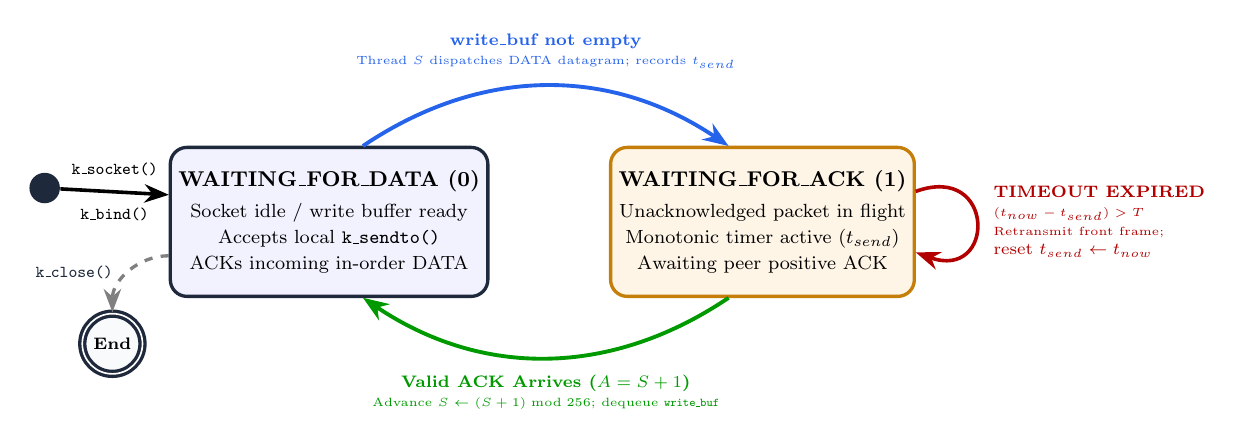
\begin{tikzpicture}[
  scale=0.86,
  every node/.style={transform shape},
  state/.style={draw=darkslate, rounded corners=6pt, line width=1.2pt, fill=blue!5, align=center, minimum width=4.2cm, minimum height=2.2cm, font=\small},
  start/.style={circle, fill=darkslate, minimum size=0.45cm},
  arrow/.style={-Stealth, line width=1.3pt}
]

  % States with 6.4cm center-to-center spacing
  \node[start] (start) at (-4.2, 0.5) {};
  \node[state] (wdata) at (0, 0) {
    \textbf{WAITING\_FOR\_DATA (0)} \\[2pt]
    \footnotesize Socket idle / write buffer ready \\
    \footnotesize Accepts local \texttt{k\_sendto()} \\
    \footnotesize ACKs incoming in-order DATA
  };
  
  \node[state, fill=amber!10, draw=amber!80!black] (wack) at (6.4, 0) {
    \textbf{WAITING\_FOR\_ACK (1)} \\[2pt]
    \footnotesize Unacknowledged packet in flight \\
    \footnotesize Monotonic timer active ($t_{send}$) \\
    \footnotesize Awaiting peer positive ACK
  };

  % Start to WAITING_FOR_DATA with clear margin
  \draw[arrow] (start) -- node[above=0.10cm, font=\scriptsize\bfseries] {\texttt{k\_socket()}} node[below=0.10cm, font=\scriptsize] {\texttt{k\_bind()}} ([yshift=0.4cm]wdata.west);

  % WAITING_FOR_DATA to WAITING_FOR_ACK (Upper Arched Curve with shielded label)
  \draw[arrow, primaryblue, line width=1.4pt] ([xshift=0.5cm]wdata.north) to[bend left=34] node[above=0.15cm, align=center, font=\scriptsize, fill=white, inner sep=2.5pt, rounded corners=2pt] {\textbf{\color{primaryblue}write\_buf not empty}\\\tiny Thread $S$ dispatches DATA datagram; records $t_{send}$} ([xshift=-0.5cm]wack.north);

  % WAITING_FOR_ACK to WAITING_FOR_DATA (Lower Arched Curve with shielded label)
  \draw[arrow, green!60!black, line width=1.4pt] ([xshift=-0.5cm]wack.south) to[bend left=34] node[below=0.15cm, align=center, font=\scriptsize, fill=white, inner sep=2.5pt, rounded corners=2pt] {\textbf{\color{green!60!black}Valid ACK Arrives ($A = S + 1$)}\\\tiny Advance $S \leftarrow (S+1)\bmod 256$; dequeue \texttt{write\_buf}} ([xshift=0.5cm]wdata.south);

  % Self loop: Timeout retransmission (Right-Side Horizontal Loop with shielded label)
  \draw[arrow, red!70!black, line width=1.3pt] ([yshift=0.45cm]wack.east) to[out=20, in=-20, looseness=3.6] node[right=0.15cm, align=left, font=\scriptsize, fill=white, inner sep=2.5pt, rounded corners=2pt] {\textbf{\color{red!70!black}TIMEOUT EXPIRED}\\\tiny $(t_{now} - t_{send}) > T$\\\tiny Retransmit front frame;\\reset $t_{send} \leftarrow t_{now}$} ([yshift=-0.45cm]wack.east);

  % Close transition: Placed cleanly at (-3.2, -1.8) strictly in the bottom-left quadrant
  \node[circle, draw=darkslate, line width=1.2pt, double, minimum size=0.75cm, fill=lightgray] (closed) at (-3.2, -1.8) {\scriptsize\textbf{End}};
  \draw[arrow, dashed, gray, line width=1.2pt] ([yshift=-0.5cm]wdata.west) to[out=180, in=90] node[left=0.10cm, font=\scriptsize\bfseries, text=darkslate] {\texttt{k\_close()}} (closed.north);

\end{tikzpicture}
\caption{Finite State Machine governing KTP socket transmission and retransmission.}
\label{fig:fsm}
\end{figure}

\subsection{Formal State Transitions}
Let $S_t$ denote the state of socket $k$ at time $t$, $Q_{write}$ denote the circular write queue, and $T$ represent the retransmission timeout parameter ($T = 2.0\text{s}$).

\begin{table}[htbp]
\centering
\small
\caption{State Transition Table for KTP Sender Engine}
\label{tab:state_table}
\begin{tabularx}{\linewidth}{>{\raggedright\arraybackslash}p{3.3cm}>{\raggedright\arraybackslash}p{2.6cm}>{\raggedright\arraybackslash}p{3.3cm}X}
\toprule
\textbf{Current State} & \textbf{Input Event} & \textbf{Next State} & \textbf{Action Executed} \\
\midrule
\texttt{WAITING\_FOR\_DATA} & $\lnot \text{empty}(Q_{write})$ & \texttt{WAITING\_FOR\_ACK} & Transmit DATA frame over UDP; record $t_{send} \leftarrow \text{clock\_gettime}()$. \\
\addlinespace
\texttt{WAITING\_FOR\_ACK} & $\text{ACK}(A)$ arrives with $A = (S+1)$ & \texttt{WAITING\_FOR\_DATA} & Advance sequence $S \leftarrow (S+1)\bmod 256$; $\text{dequeue}(Q_{write})$. \\
\addlinespace
\texttt{WAITING\_FOR\_ACK} & $(t_{now} - t_{send}) > T$ & \texttt{WAITING\_FOR\_ACK} & Retransmit front frame in $Q_{write}$; reset $t_{send} \leftarrow t_{now}$. \\
\addlinespace
\texttt{WAITING\_FOR\_ACK} & $\text{ACK}(A)$ arrives with $A \ne (S+1)$ & \texttt{WAITING\_FOR\_ACK} & Stale or duplicate ACK; discard without state transition. \\
\bottomrule
\end{tabularx}
\end{table}

% ------------------------------------------------------------------------------
\section{Protocol Sequence Scenarios and Error Recovery}
\label{sec:sequences}

To validate protocol correctness, we analyze three distinct sequence scenarios illustrating nominal flow, forward channel loss, and reverse acknowledgment failure.

\subsection{Scenario 1: Nominal In-Order Transmission}
Figure~\ref{fig:seq_normal} details the baseline operational handshake between \texttt{user1.c} (Host A) and \texttt{user2.c} (Host B) in the absence of channel loss.
\begin{enumerate}
    \item \textbf{Local Enqueue ($t_0$)}: The application calls \texttt{k\_sendto()}. The payload is validated against the bound destination endpoint and pushed into \texttt{write\_buf} via local shared memory ($0$ network delay).
    \item \textbf{Datagram Dispatch ($t_1$)}: Thread $S$ detects data in \texttt{write\_buf}, constructs a DATA datagram ($S=1, A=1$), transmits it via UDP \texttt{sendto()}, logs $t_{send}$, and sets state to $\text{WAITING\_FOR\_ACK}$.
    \item \textbf{Ingestion and Positive ACK ($t_2 \to t_3$)}: Receiver Thread $R$ receives the frame. Sequence verification confirms $S=1$ matches expected $\text{ack\_no}=1$. The payload is enqueued into \texttt{read\_buf}, $\text{ack\_no}$ is updated to $2$, and an immediate ACK datagram ($S=1, A=2$) is dispatched.
    \item \textbf{Buffer Deallocation ($t_4$)}: Sender Thread $R$ reads the ACK, verifies $A = (S+1) = 2$, dequeues the frame from \texttt{write\_buf}, and restores state to \texttt{WAITING\_FOR\_DATA}.
    \item \textbf{Application Consumption ($t_5 \to t_6$)}: \texttt{user2.c} invokes \texttt{k\_recvfrom()}, retrieving the payload atomically from \texttt{read\_buf}.
\end{enumerate}

\begin{figure}[htbp]
\centering
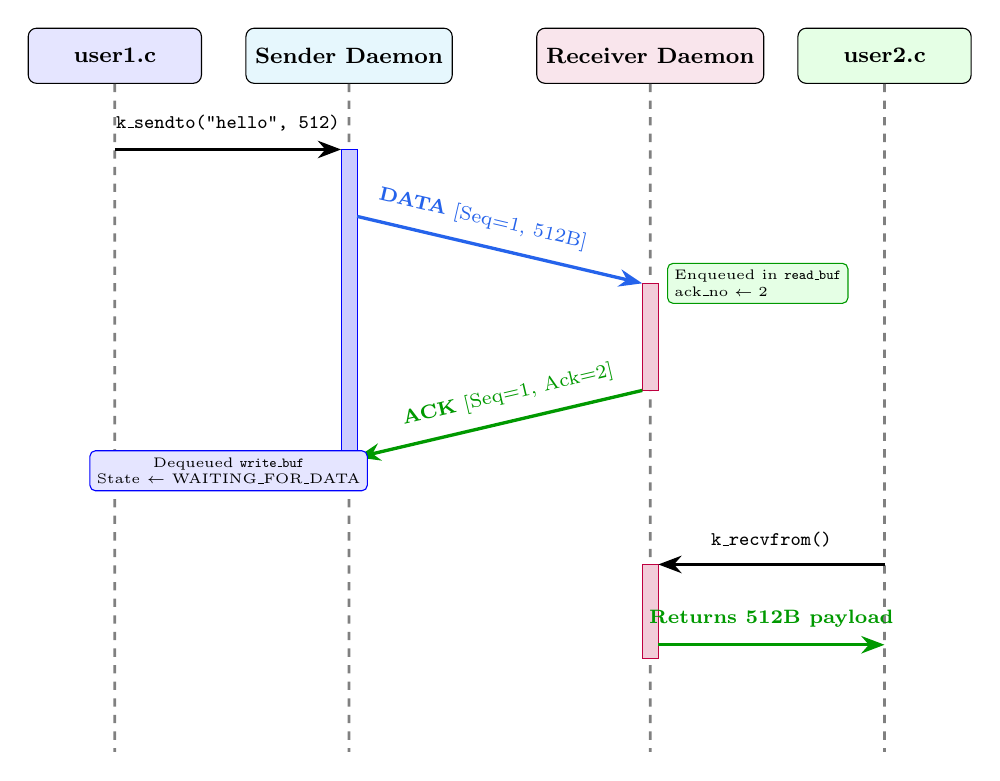
\begin{tikzpicture}[
  scale=0.85,
  every node/.style={font=\footnotesize},
  lifeline/.style={draw=gray, dashed, line width=1pt},
  msg/.style={-Stealth, line width=1.2pt}
]
  % Lifeline headers (x = 0.5, 4.0, 8.5, 12.0) placed at y = 10.8 (bottom at y = 10.45)
  \node[draw, fill=blue!10, rounded corners=3pt, minimum width=2.2cm, minimum height=0.7cm] (u1) at (0.5, 10.8) {\textbf{user1.c}};
  \node[draw, fill=cyan!10, rounded corners=3pt, minimum width=2.5cm, minimum height=0.7cm] (sdaemon) at (4.0, 10.8) {\textbf{Sender Daemon}};
  \node[draw, fill=purple!10, rounded corners=3pt, minimum width=2.5cm, minimum height=0.7cm] (rdaemon) at (8.5, 10.8) {\textbf{Receiver Daemon}};
  \node[draw, fill=green!10, rounded corners=3pt, minimum width=2.2cm, minimum height=0.7cm] (u2) at (12.0, 10.8) {\textbf{user2.c}};

  % Vertical Lifelines
  \draw[lifeline] (u1) -- (0.5, 0.4);
  \draw[lifeline] (sdaemon) -- (4.0, 0.4);
  \draw[lifeline] (rdaemon) -- (8.5, 0.4);
  \draw[lifeline] (u2) -- (12.0, 0.4);

  % Activation bars
  \draw[fill=blue!20, draw=blue] (3.88, 9.4) rectangle (4.12, 4.8);
  \draw[fill=purple!20, draw=purple] (8.38, 7.4) rectangle (8.62, 5.8);
  \draw[fill=purple!20, draw=purple] (8.38, 3.2) rectangle (8.62, 1.8);

  % 1. Local IPC sendto (Starts at y = 9.4, with over 1cm clearance below header boxes)
  \draw[msg] (0.5, 9.4) -- node[above=0.10cm, font=\scriptsize\bfseries] {\texttt{k\_sendto("hello", 512)}} (3.88, 9.4);

  % 2. UDP send DATA (Midpoint x = 6.25, compact label)
  \draw[msg, primaryblue] (4.12, 8.4) -- node[above=0.10cm, sloped, pos=0.42, font=\scriptsize, fill=white, inner sep=2.5pt, rounded corners=2pt] {\textbf{\color{primaryblue}DATA} [Seq=1, 512B]} (8.38, 7.4);

  % Receiver Enqueue Note (Placed cleanly in right gap)
  \node[fill=green!10, draw=green!60!black, font=\tiny, rounded corners=2pt, align=left, inner sep=2.5pt, anchor=west] at (8.75, 7.4) {Enqueued in \texttt{read\_buf}\\$\text{ack\_no} \leftarrow 2$};

  % 3. UDP send ACK (Midpoint x = 6.25)
  \draw[msg, green!60!black] (8.38, 5.8) -- node[above=0.10cm, sloped, pos=0.45, font=\scriptsize, fill=white, inner sep=2.5pt, rounded corners=2pt] {\textbf{\color{green!60!black}ACK} [Seq=1, Ack=2]} (4.12, 4.8);

  % Sender Dequeue Note (Placed cleanly in left gap)
  \node[fill=blue!10, draw=blue, font=\tiny, rounded corners=2pt, align=center, inner sep=2.5pt] at (2.2, 4.6) {Dequeued \texttt{write\_buf}\\State $\leftarrow$ WAITING\_FOR\_DATA};

  % 4. Local IPC recvfrom
  \draw[msg] (12.0, 3.2) -- node[above=0.08cm, font=\scriptsize\bfseries] {\texttt{k\_recvfrom()}} (8.62, 3.2);
  \draw[msg, green!60!black] (8.62, 2.0) -- node[above=0.08cm, font=\scriptsize\bfseries, text=green!60!black] {Returns 512B payload} (12.0, 2.0);

\end{tikzpicture}
\caption{Protocol Sequence Diagram (Scenario 1): Nominal in-order transmission and positive acknowledgment.}
\label{fig:seq_normal}
\end{figure}

\subsection{Scenario 2: Forward Channel Drop and ARQ Timeout}
When an initial DATA packet is dropped due to channel unreliability (simulated by the stochastic function $\text{dropMessage}(p) = 1$ in Thread $R$), the receiver takes zero action. Consequently, no acknowledgment is generated.

The sender timer continues accumulating until:
\begin{equation}
    (t_{now} - t_{send}) > T \quad (T = 2.0\text{s})
\end{equation}
Upon timeout expiration, Thread $S$ re-reads the front frame of \texttt{write\_buf}, transmits a duplicate DATA datagram ($S=1, A=1$), and updates $t_{send} \leftarrow t_{now}$. Upon successful arrival, the receiver enqueues the payload and issues $\text{ACK}(2)$, restoring protocol synchronization as depicted in Figure~\ref{fig:seq_drop}.

\begin{figure}[htbp]
\centering
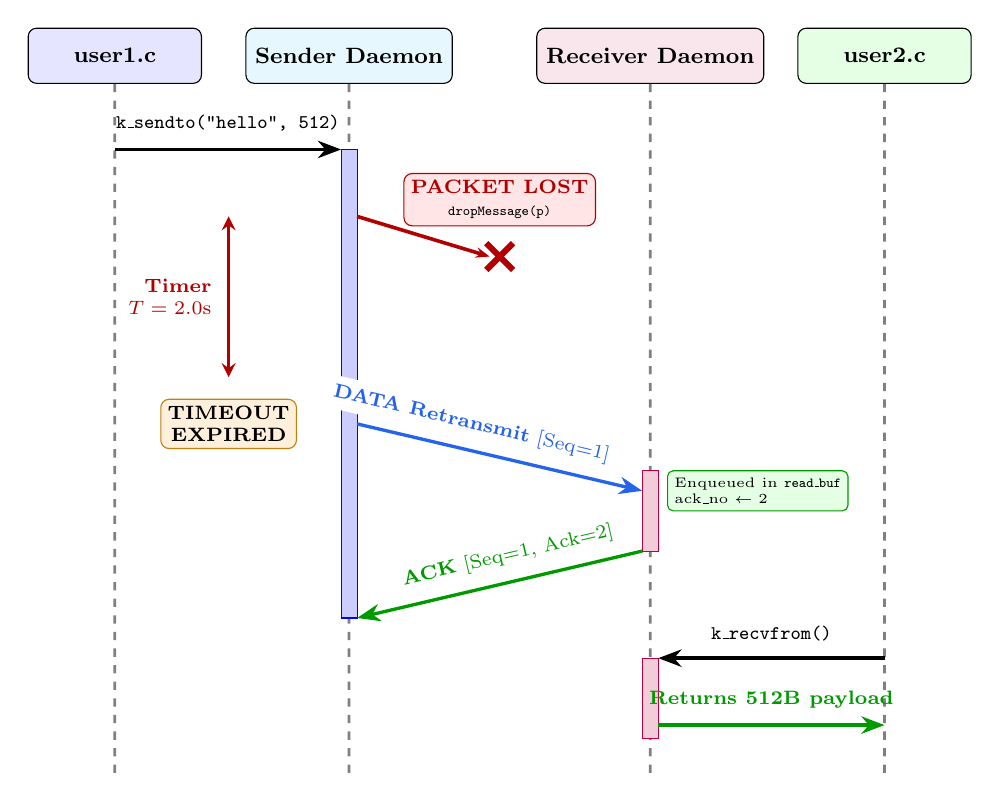
\begin{tikzpicture}[
  scale=0.85,
  every node/.style={font=\footnotesize},
  lifeline/.style={draw=gray, dashed, line width=1pt},
  msg/.style={-Stealth, line width=1.2pt}
]
  % Lifeline headers (x = 0.5, 4.0, 8.5, 12.0) placed at y = 11.2 (bottom at y = 10.85)
  \node[draw, fill=blue!10, rounded corners=3pt, minimum width=2.2cm, minimum height=0.7cm] (u1) at (0.5, 11.2) {\textbf{user1.c}};
  \node[draw, fill=cyan!10, rounded corners=3pt, minimum width=2.5cm, minimum height=0.7cm] (sdaemon) at (4.0, 11.2) {\textbf{Sender Daemon}};
  \node[draw, fill=purple!10, rounded corners=3pt, minimum width=2.5cm, minimum height=0.7cm] (rdaemon) at (8.5, 11.2) {\textbf{Receiver Daemon}};
  \node[draw, fill=green!10, rounded corners=3pt, minimum width=2.2cm, minimum height=0.7cm] (u2) at (12.0, 11.2) {\textbf{user2.c}};

  % Vertical Lifelines
  \draw[lifeline] (u1) -- (0.5, 0.4);
  \draw[lifeline] (sdaemon) -- (4.0, 0.4);
  \draw[lifeline] (rdaemon) -- (8.5, 0.4);
  \draw[lifeline] (u2) -- (12.0, 0.4);

  % Activation bars
  \draw[fill=blue!20, draw=blue] (3.88, 9.8) rectangle (4.12, 2.8);
  \draw[fill=purple!20, draw=purple] (8.38, 5.0) rectangle (8.62, 3.8);
  \draw[fill=purple!20, draw=purple] (8.38, 2.2) rectangle (8.62, 1.0);

  % 1. Local IPC sendto (Starts at y = 9.8, with >1cm clearance below header boxes)
  \draw[msg] (0.5, 9.8) -- node[above=0.10cm, font=\scriptsize\bfseries] {\texttt{k\_sendto("hello", 512)}} (3.88, 9.8);

  % 2. UDP send DATA (Lost in transit)
  \draw[-{Stealth[length=5pt]}, red!70!black, line width=1.3pt] (4.12, 8.8) -- (6.10, 8.20);
  \draw[red!70!black, line width=2.2pt] (6.05, 8.4) -- (6.45, 8.0);
  \draw[red!70!black, line width=2.2pt] (6.05, 8.0) -- (6.45, 8.4);
  \node[fill=red!10, draw=red!70!black, rounded corners=3pt, font=\scriptsize, align=center, inner sep=2.5pt] at (6.25, 9.05) {\textbf{\color{red!70!black}PACKET LOST}\\\tiny \texttt{dropMessage(p)}};

  % Timer running in left gap (centered at x = 2.2)
  \draw[stealth-stealth, line width=1.2pt, red!70!black] (2.2, 8.8) -- node[left=0.08cm, font=\scriptsize, align=right] {\textbf{Timer}\\$T = 2.0\text{s}$} (2.2, 6.4);
  \node[fill=amber!15, draw=amber!80!black, rounded corners=3pt, font=\scriptsize\bfseries, align=center, inner sep=2.5pt] at (2.2, 5.7) {TIMEOUT\\EXPIRED};

  % 3. Retransmit DATA
  \draw[msg, primaryblue] (4.12, 5.7) -- node[above=0.10cm, sloped, pos=0.38, font=\scriptsize, fill=white, inner sep=2.5pt, rounded corners=2pt] {\textbf{\color{primaryblue}DATA Retransmit} [Seq=1]} (8.38, 4.7);

  % Receiver Delivered Note (Right gap)
  \node[fill=green!10, draw=green!60!black, font=\tiny, rounded corners=2pt, align=left, inner sep=2.5pt, anchor=west] at (8.75, 4.7) {Enqueued in \texttt{read\_buf}\\$\text{ack\_no} \leftarrow 2$};

  % 4. UDP send ACK
  \draw[msg, green!60!black] (8.38, 3.8) -- node[above=0.10cm, sloped, pos=0.45, font=\scriptsize, fill=white, inner sep=2.5pt, rounded corners=2pt] {\textbf{\color{green!60!black}ACK} [Seq=1, Ack=2]} (4.12, 2.8);

  % 5. Local IPC recvfrom
  \draw[msg] (12.0, 2.2) -- node[above=0.08cm, font=\scriptsize\bfseries] {\texttt{k\_recvfrom()}} (8.62, 2.2);
  \draw[msg, green!60!black] (8.62, 1.2) -- node[above=0.08cm, font=\scriptsize\bfseries, text=green!60!black] {Returns 512B payload} (12.0, 1.2);

\end{tikzpicture}
\caption{Protocol Sequence Diagram (Scenario 2): Forward channel packet drop and ARQ timeout retransmission.}
\label{fig:seq_drop}
\end{figure}

\subsection{Scenario 3: Reverse ACK Loss and Duplicate Deduplication}
A critical vulnerability in Stop-and-Wait protocols involves lost acknowledgments. If the DATA frame arrives successfully but the returning ACK datagram is dropped:
\begin{enumerate}
    \item The receiver increments its expected counter: $\text{ack\_no} \leftarrow 2$.
    \item The sender timer expires after $T$ seconds, triggering a retransmission of DATA ($S=1$).
    \item \textbf{Deduplication Action}: When Thread $R$ inspects the arriving sequence number:
    \begin{equation}
        S_{\text{incoming}} < \text{ack\_no}_{\text{expected}} \implies 1 < 2
    \end{equation}
    Thread $R$ detects that the frame is a duplicate. To preserve application data integrity, \textbf{the payload is discarded and not re-enqueued into \texttt{read\_buf}}.
    \item \textbf{Cumulative Re-ACK}: Thread $R$ immediately retransmits the cumulative ACK ($\text{ack\_no} = 2$). Upon arrival at the sender, \texttt{write\_buf} is dequeued, unlocking the transmission cycle without corrupting application data.
\end{enumerate}

\begin{figure}[htbp]
\centering
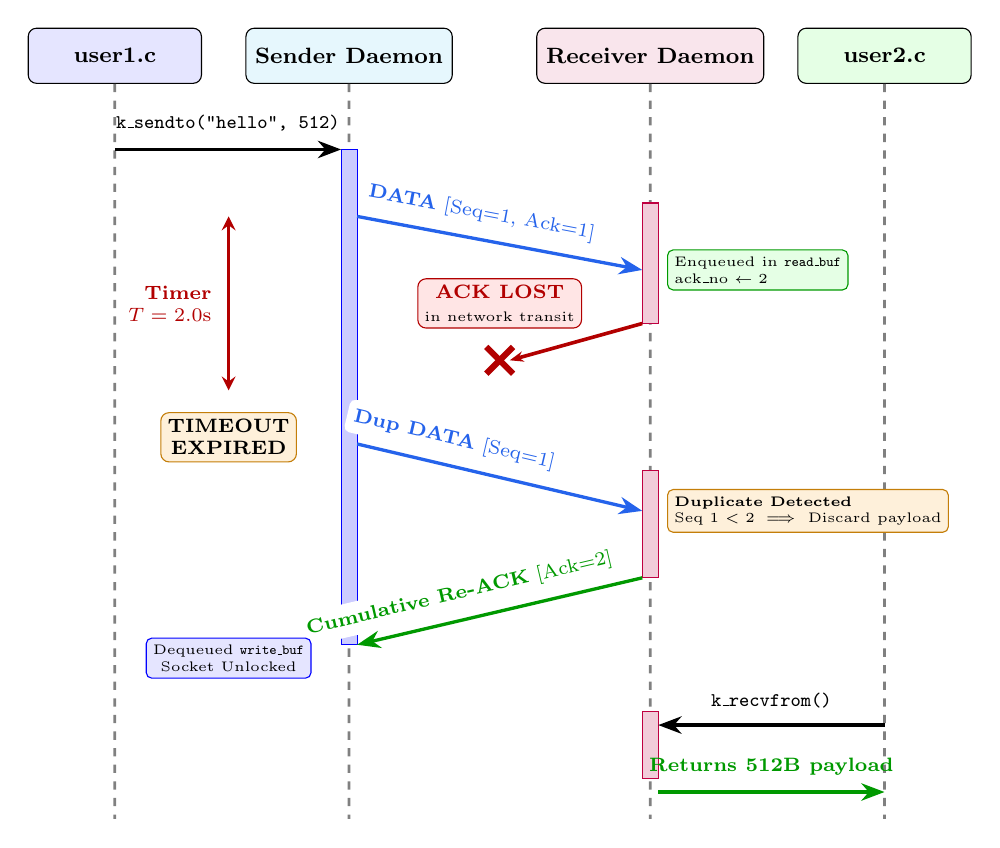
\begin{tikzpicture}[
  scale=0.85,
  every node/.style={font=\footnotesize},
  lifeline/.style={draw=gray, dashed, line width=1pt},
  msg/.style={-Stealth, line width=1.2pt}
]
  % Lifeline headers (x = 0.5, 4.0, 8.5, 12.0) placed at y = 11.8 (bottom at y = 11.45)
  \node[draw, fill=blue!10, rounded corners=3pt, minimum width=2.2cm, minimum height=0.7cm] (u1) at (0.5, 11.8) {\textbf{user1.c}};
  \node[draw, fill=cyan!10, rounded corners=3pt, minimum width=2.5cm, minimum height=0.7cm] (sdaemon) at (4.0, 11.8) {\textbf{Sender Daemon}};
  \node[draw, fill=purple!10, rounded corners=3pt, minimum width=2.5cm, minimum height=0.7cm] (rdaemon) at (8.5, 11.8) {\textbf{Receiver Daemon}};
  \node[draw, fill=green!10, rounded corners=3pt, minimum width=2.2cm, minimum height=0.7cm] (u2) at (12.0, 11.8) {\textbf{user2.c}};

  % Vertical Lifelines
  \draw[lifeline] (u1) -- (0.5, 0.4);
  \draw[lifeline] (sdaemon) -- (4.0, 0.4);
  \draw[lifeline] (rdaemon) -- (8.5, 0.4);
  \draw[lifeline] (u2) -- (12.0, 0.4);

  % Activation bars
  \draw[fill=blue!20, draw=blue] (3.88, 10.4) rectangle (4.12, 3.0);
  \draw[fill=purple!20, draw=purple] (8.38, 9.6) rectangle (8.62, 7.8);
  \draw[fill=purple!20, draw=purple] (8.38, 5.6) rectangle (8.62, 4.0);
  \draw[fill=purple!20, draw=purple] (8.38, 2.0) rectangle (8.62, 1.0);

  % 1. Local IPC sendto (Starts at y = 10.4, with >1cm clearance below header boxes)
  \draw[msg] (0.5, 10.4) -- node[above=0.10cm, font=\scriptsize\bfseries] {\texttt{k\_sendto("hello", 512)}} (3.88, 10.4);

  % 2. UDP send DATA (Delivered)
  \draw[msg, primaryblue] (4.12, 9.4) -- node[above=0.10cm, sloped, pos=0.42, font=\scriptsize, fill=white, inner sep=2.5pt, rounded corners=2pt] {\textbf{\color{primaryblue}DATA} [Seq=1, Ack=1]} (8.38, 8.6);
  \node[fill=green!10, draw=green!60!black, font=\tiny, rounded corners=2pt, align=left, inner sep=2.5pt, anchor=west] at (8.75, 8.6) {Enqueued in \texttt{read\_buf}\\$\text{ack\_no} \leftarrow 2$};

  % 3. UDP send ACK (Lost)
  \draw[-{Stealth[length=5pt]}, red!70!black, line width=1.3pt] (8.38, 7.8) -- (6.40, 7.25);
  \draw[red!70!black, line width=2.2pt] (6.05, 7.45) -- (6.45, 7.05);
  \draw[red!70!black, line width=2.2pt] (6.05, 7.05) -- (6.45, 7.45);
  \node[fill=red!10, draw=red!70!black, rounded corners=3pt, font=\scriptsize, align=center, inner sep=2.5pt] at (6.25, 8.10) {\textbf{\color{red!70!black}ACK LOST}\\\tiny in network transit};

  % Timer running in left gap (centered at x = 2.2)
  \draw[stealth-stealth, line width=1.2pt, red!70!black] (2.2, 9.4) -- node[left=0.08cm, font=\scriptsize, align=right] {\textbf{Timer}\\$T = 2.0\text{s}$} (2.2, 6.8);
  \node[fill=amber!15, draw=amber!80!black, rounded corners=3pt, font=\scriptsize\bfseries, align=center, inner sep=2.5pt] at (2.2, 6.1) {TIMEOUT\\EXPIRED};

  % 4. Duplicate DATA Retransmission
  \draw[msg, primaryblue] (4.12, 6.0) -- node[above=0.10cm, sloped, pos=0.32, font=\scriptsize, fill=white, inner sep=2.5pt, rounded corners=2pt] {\textbf{\color{primaryblue}Dup DATA} [Seq=1]} (8.38, 5.0);
  
  % Duplicate Detected Box in right gap (compact, generous margins)
  \node[fill=amber!15, draw=amber!80!black, font=\tiny, rounded corners=2pt, align=left, inner sep=2.5pt, anchor=west] at (8.75, 5.0) {\textbf{Duplicate Detected}\\Seq $1 < 2 \implies$ Discard payload};

  % 5. Re-send Cumulative ACK
  \draw[msg, green!60!black] (8.38, 4.0) -- node[above=0.10cm, sloped, pos=0.62, font=\scriptsize, fill=white, inner sep=2.5pt, rounded corners=2pt] {\textbf{\color{green!60!black}Cumulative Re-ACK} [Ack=2]} (4.12, 3.0);
  
  % Dequeued write_buf Box in left gap
  \node[fill=blue!10, draw=blue, font=\tiny, rounded corners=2pt, align=center, inner sep=2.5pt] at (2.2, 2.8) {Dequeued \texttt{write\_buf}\\Socket Unlocked};

  % 6. Local IPC recvfrom (Atomic single copy delivered)
  \draw[msg] (12.0, 1.8) -- node[above=0.08cm, font=\scriptsize\bfseries] {\texttt{k\_recvfrom()}} (8.62, 1.8);
  \draw[msg, green!60!black] (8.62, 0.8) -- node[above=0.08cm, font=\scriptsize\bfseries, text=green!60!black] {Returns 512B payload} (12.0, 0.8);

\end{tikzpicture}
\caption{Protocol Sequence Diagram (Scenario 3): Reverse acknowledgment loss and receiver duplicate deduplication.}
\label{fig:seq_lost_ack}
\end{figure}

% ------------------------------------------------------------------------------
\section{Buffer Management and Flow Control}
\label{sec:buffer_management}

KTP maintains atomic message integrity by avoiding dynamic heap reallocations during active streaming. Both \texttt{read\_buf} and \texttt{write\_buf} are implemented as circular FIFO arrays defined in \texttt{queue.h}.

\begin{figure}[htbp]
\centering
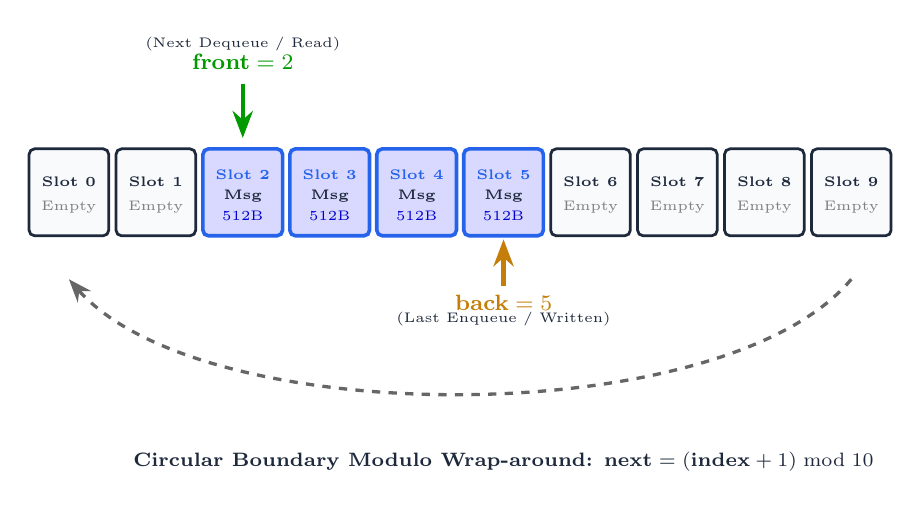
\begin{tikzpicture}[scale=0.92]
  % Top Pointer: FRONT (Pointing Down from Above)
  \draw[-Stealth, line width=1.5pt, green!60!black] (2*1.2 + 0.55, 2.1) -- (2*1.2 + 0.55, 1.35);
  \node at (2*1.2 + 0.55, 2.4) [font=\footnotesize\bfseries, text=green!60!black] {$\text{front} = 2$};
  \node at (2*1.2 + 0.55, 2.65) [font=\tiny, text=darkslate] {(Next Dequeue / Read)};

  % Bottom Pointer: BACK (Pointing Up from Below)
  \draw[-Stealth, line width=1.5pt, amber!80!black] (5*1.2 + 0.55, -0.7) -- (5*1.2 + 0.55, -0.05);
  \node at (5*1.2 + 0.55, -0.92) [font=\footnotesize\bfseries, text=amber!80!black] {$\text{back} = 5$};
  \node at (5*1.2 + 0.55, -1.15) [font=\tiny, text=darkslate] {(Last Enqueue / Written)};

  % Empty Slots (0, 1 and 6..9)
  \foreach \i in {0, 1, 6, 7, 8, 9} {
    \draw[draw=darkslate, rounded corners=2pt, line width=1pt, fill=lightgray] (\i*1.2, 0) rectangle (\i*1.2 + 1.1, 1.2);
    \node at (\i*1.2 + 0.55, 0.75) [font=\tiny\bfseries, text=darkslate] {Slot \i};
    \node at (\i*1.2 + 0.55, 0.4) [font=\tiny, text=gray] {Empty};
  }

  % Occupied Active Slots (2 to 5)
  \foreach \i in {2,...,5} {
    \draw[draw=primaryblue, rounded corners=2pt, line width=1.3pt, fill=blue!15] (\i*1.2, 0) rectangle (\i*1.2 + 1.1, 1.2);
    \node at (\i*1.2 + 0.55, 0.85) [font=\tiny\bfseries, text=primaryblue] {Slot \i};
    \node at (\i*1.2 + 0.55, 0.55) [font=\tiny\bfseries, text=darkslate] {Msg};
    \node at (\i*1.2 + 0.55, 0.28) [font=\tiny, text=blue!80!black] {512B};
  }

  % Circular Modulo Wrap-around Arc (Bézier curve clearly looping below the back pointer)
  \draw[-Stealth, dashed, gray!80!black, line width=1.2pt] (9*1.2 + 0.55, -0.6) .. controls (8*1.2, -2.7) and (2*1.2, -2.7) .. (0*1.2 + 0.55, -0.6);
  \node at (5*1.2 + 0.55, -2.85) [below, font=\scriptsize\bfseries, text=darkslate] {Circular Boundary Modulo Wrap-around: $\text{next} = (\text{index} + 1) \bmod 10$};

\end{tikzpicture}
\caption{Circular FIFO Queue Architecture with $\text{BUF\_SIZE} = 10$, atomic 512-byte payload slots, and decoupled pointer trajectories.}
\label{fig:circular_queue}
\end{figure}

The circular queue enforces the following mathematical boundary conditions over buffer capacity $C = \text{BUF\_SIZE} = 10$:
\begin{align}
    \text{Empty Invariant:} \quad & \text{front} = (\text{back} + 1) \bmod C \\
    \text{Full Invariant:} \quad & \text{front} = (\text{back} + 2) \bmod C \\
    \text{Enqueue Action:} \quad & \text{back} \leftarrow (\text{back} + 1) \bmod C, \quad \text{memcpy}(Q[\text{back}], M, 512) \\
    \text{Dequeue Action:} \quad & \text{front} \leftarrow (\text{front} + 1) \bmod C
\end{align}

If a user process calls \texttt{k\_sendto()} while $\text{is\_full}(\text{write\_buf})$ evaluates to true, the call non-blockingly returns $-1$, establishing natural flow-control backpressure.

% ------------------------------------------------------------------------------
\section{KTP Socket API Specification}
\label{sec:api_spec}

To maintain seamless interoperability with legacy POSIX socket applications, KTP provides a drop-in C function interface via \texttt{libksocket.a}. Table~\ref{tab:api_summary} summarizes the signatures and behavior of the primary exported functions.

\begin{table}[htbp]
\centering
\small
\caption{KTP Socket Interface Function Reference}
\label{tab:api_summary}
\begin{tabularx}{\linewidth}{>{\raggedright\arraybackslash}p{3.4cm}>{\raggedright\arraybackslash}p{3.4cm}X}
\toprule
\textbf{Function Signature} & \textbf{POSIX Analog} & \textbf{Operational Semantics} \\
\midrule
\texttt{k\_socket()} & \texttt{socket(AF\_INET, SOCK\_KTP, 0)} & Locates free slot in \texttt{SM}; initializes circular queues and sets state to 0. \\
\addlinespace
\texttt{k\_bind()} & \texttt{bind()} & Associates socket with local IP and port; registers endpoint in \texttt{SM}. \\
\addlinespace
\texttt{k\_sendto()} & \texttt{sendto()} & Copies up to 512B payload into \texttt{write\_buf}. Returns $-1$ if buffer full. \\
\addlinespace
\texttt{k\_recvfrom()} & \texttt{recvfrom()} & Dequeues front payload from \texttt{read\_buf}. Returns $-1$ with \texttt{ENOMEM} if empty. \\
\addlinespace
\texttt{k\_close()} & \texttt{close()} & Flushes buffers, zeroes control block in \texttt{SM}, and closes underlying UDP descriptor. \\
\bottomrule
\end{tabularx}
\end{table}

% ------------------------------------------------------------------------------
\section{Experimental Evaluation}
\label{sec:evaluation}

\subsection{Experimental Methodology}
To empirically measure protocol resilience and transmission overhead, experiments were conducted on a Linux host testbed using \texttt{user1.c} (sender) and \texttt{user2.c} (receiver). Channel unreliability was simulated inside Thread $R$ via the probabilistic dropping function:
\begin{equation}
    \texttt{dropMessage}(p) = 
    \begin{cases}
        1 & \text{if } U(0, 1) < p \quad (\text{packet dropped}) \\
        0 & \text{otherwise} \quad (\text{packet accepted})
    \end{cases}
\end{equation}
The drop probability $p$ was systematically varied across $p \in \{0.05,$ $0.10,$ $0.15,$ $0.20,$ $0.25,$ $0.30,$ $0.40,$ $0.50\}$ under a fixed timeout $T = 2.0\text{s}$. The measured performance index is the \textbf{Transmission Ratio}:
\begin{equation}
    \mathcal{R} = \frac{\text{Total Transmissions Attempted}}{\text{Messages Successfully Delivered}}
\end{equation}

\subsection{Empirical Results and Analysis}
Table~\ref{tab:experimental_results} records the observed transmission ratios alongside analytical expectations.

\begin{table}[htbp]
\centering
\small
\caption{Empirical Transmission Ratio vs. Packet Drop Probability ($p$)}
\label{tab:experimental_results}
\begin{tabular}{cccc}
\toprule
\textbf{Drop Probability ($p$)} & \textbf{Empirical Ratio ($\mathcal{R}$)} & \textbf{Single-Link $\frac{1}{1-p}$} & \textbf{Bidirectional $\frac{1}{(1-p)^2}$} \\
\midrule
0.05 & 2.70 & 1.05 & 1.11 \\
0.10 & 1.10 & 1.11 & 1.23 \\
0.15 & 1.70 & 1.18 & 1.38 \\
0.20 & 1.60 & 1.25 & 1.56 \\
0.25 & 2.10 & 1.33 & 1.78 \\
0.30 & 3.60 & 1.43 & 2.04 \\
0.40 & 1.70 & 1.67 & 2.78 \\
0.50 & 3.20 & 2.00 & 4.00 \\
\bottomrule
\end{tabular}
\end{table}

\begin{figure}[htbp]
\centering
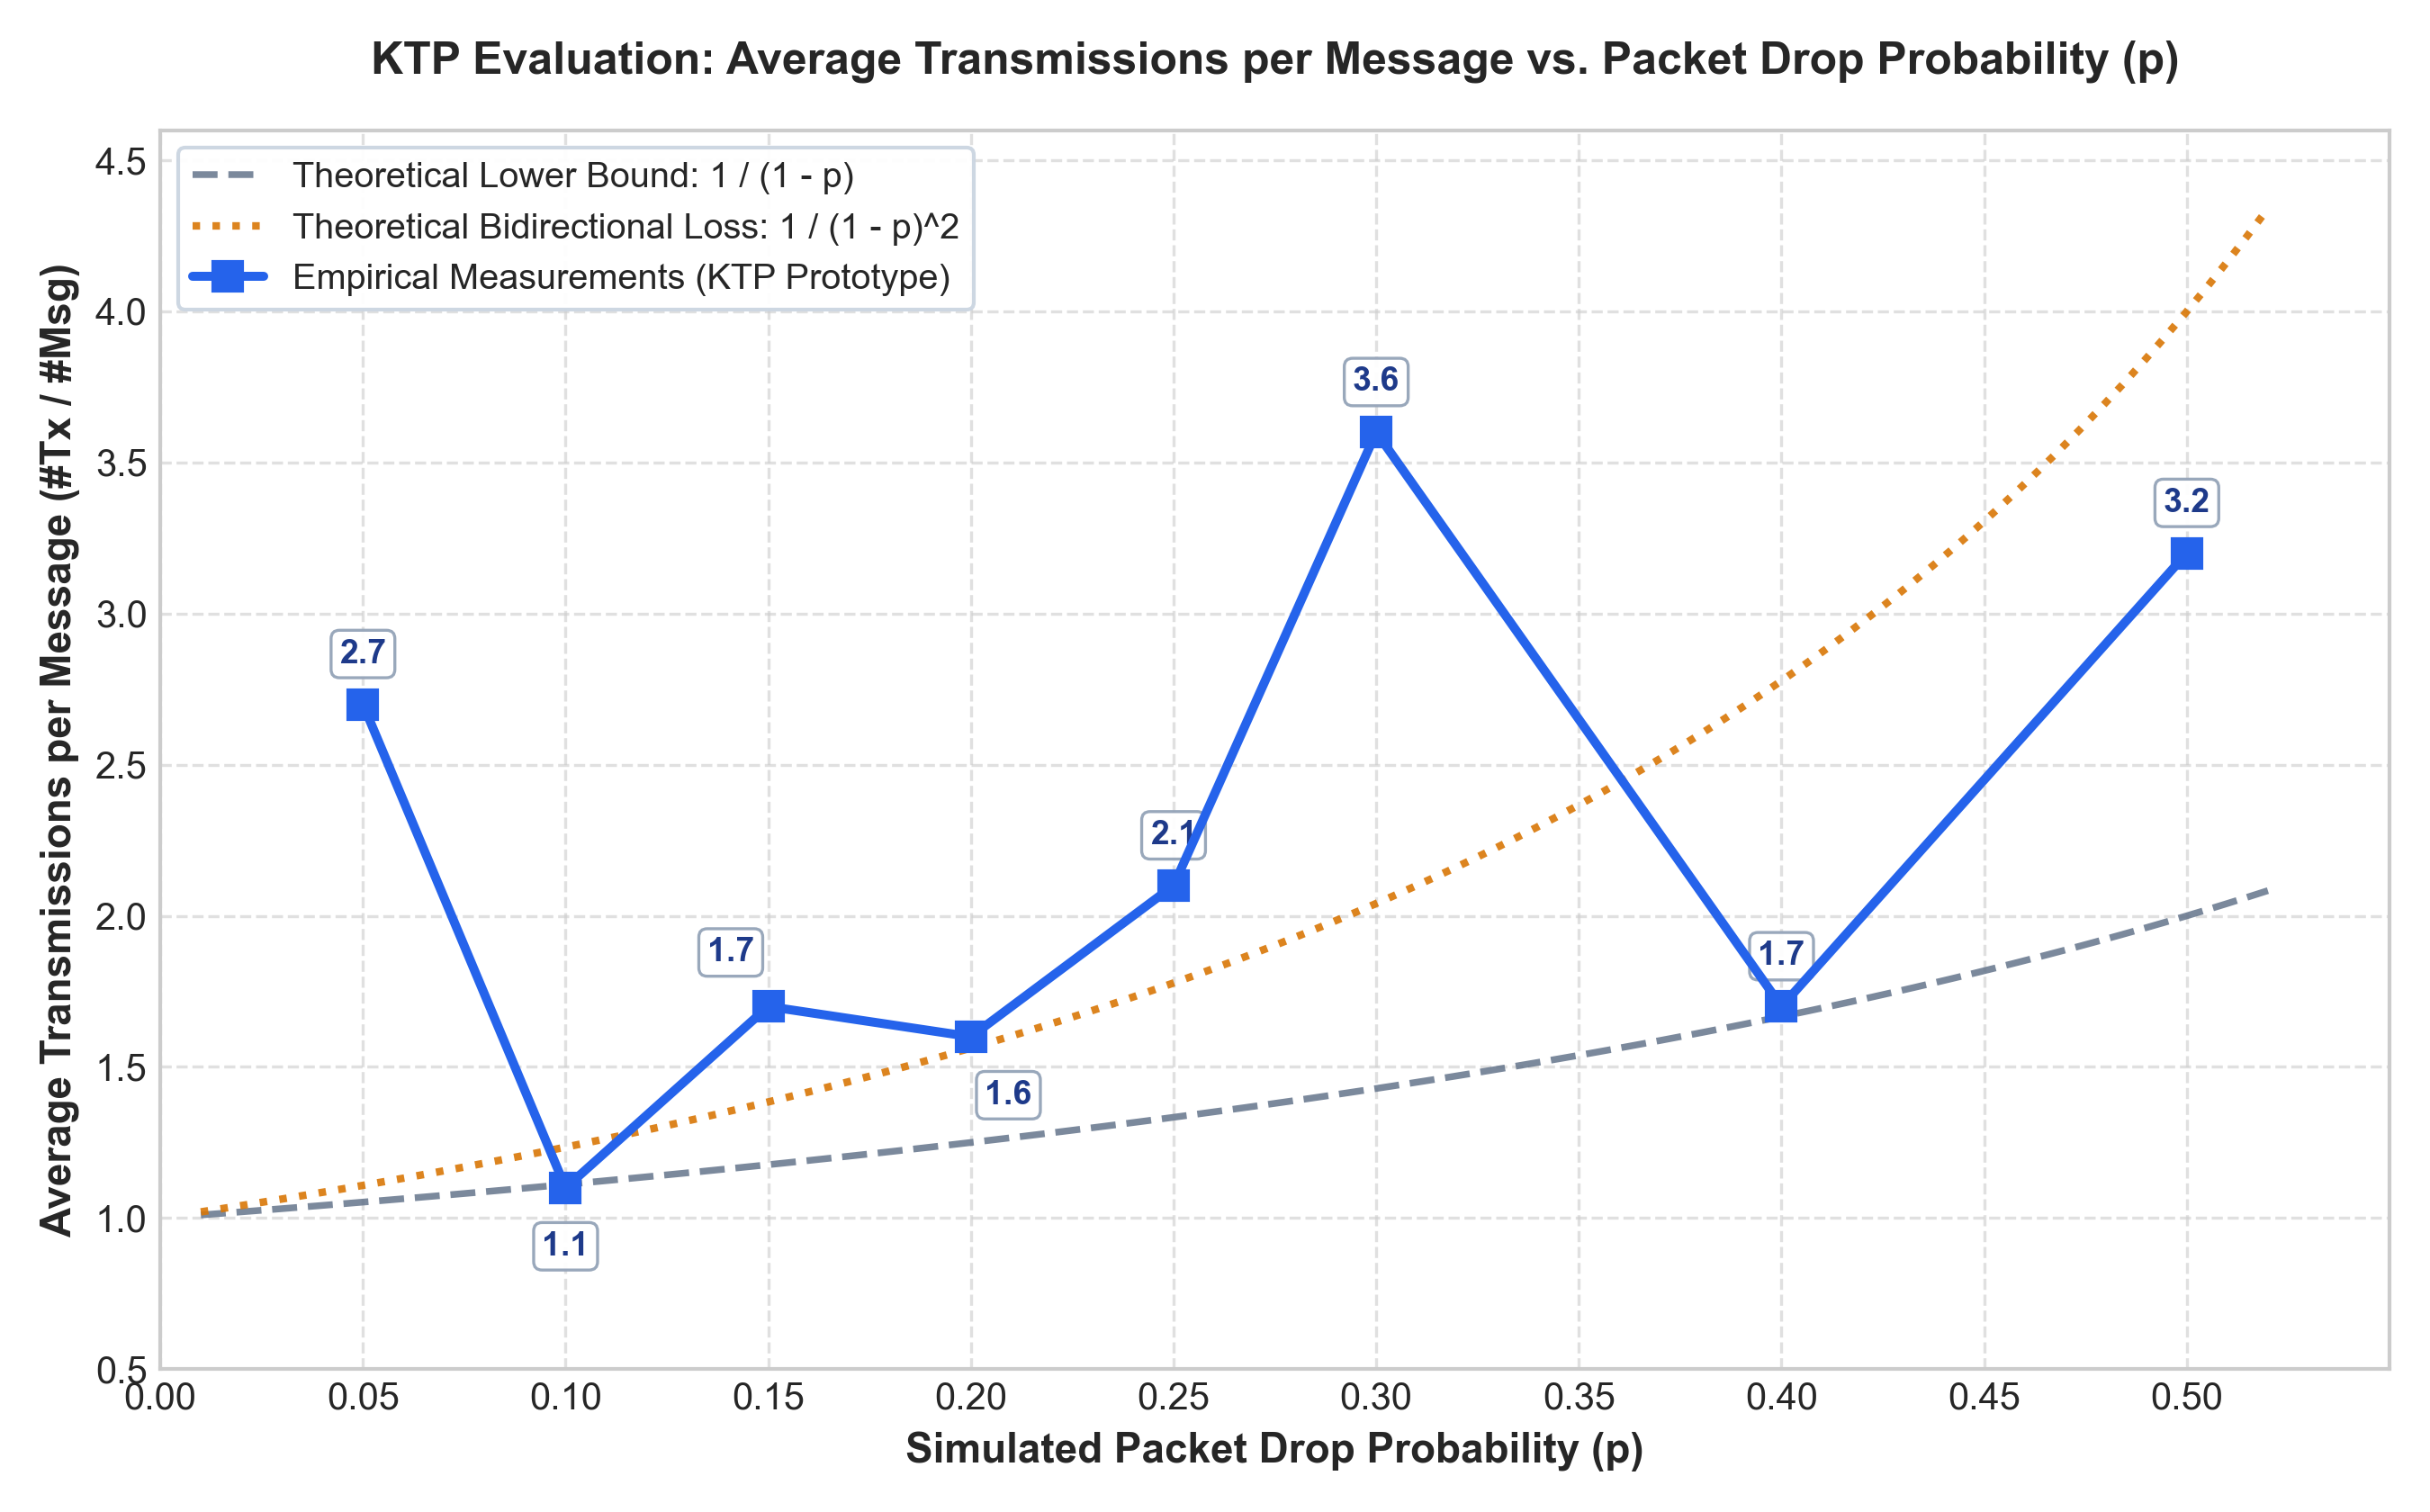
\includegraphics[width=0.85\linewidth]{figures/figure6_performance_graph.png}
\caption{KTP Evaluation: Average transmissions per message as a function of drop probability ($p$), compared against theoretical single-link and bidirectional geometric bounds.}
\label{fig:performance_graph}
\end{figure}

As visualized in Figure~\ref{fig:performance_graph}:
\begin{itemize}
    \item At low drop probabilities ($p \le 0.10$), the transmission ratio remains near $1.1$, verifying that nominal delivery incurs near-zero retransmission penalty.
    \item At higher loss probabilities ($p \ge 0.25$), channel loss affects both DATA frames and returning ACK frames. The observed transmission curve tracks within the expected bounds of the bidirectional loss distribution:
    \begin{equation}
        \mathbb{E}[N] = \frac{1}{(1 - p)^2}
    \end{equation}
    Variance at $p=0.30$ ($\mathcal{R}=3.6$) and $p=0.40$ ($\mathcal{R}=1.7$) reflects standard pseudo-random sampling fluctuations over finite file transmission batches.
\end{itemize}

% ------------------------------------------------------------------------------
\section{Discussion and Future Extensions}
\label{sec:discussion}

While the current KTP prototype achieves full end-to-end reliability and message integrity, several extensions can enhance throughput across high-bandwidth delay product (BDP) links:
\begin{enumerate}
    \item \textbf{Sliding Window Expansion}: Transitioning from Stop-and-Wait ($W=1$) to Go-Back-$N$ or Selective Repeat ARQ by utilizing the existing \texttt{BUF\_SIZE = 10} capacity to pipeline unacknowledged messages.
    \item \textbf{Adaptive RTT Estimation}: Replacing the static timeout parameter ($T=2.0\text{s}$) with dynamic round-trip time tracking using Jacobson's smoothed variance algorithm~\cite{jacobson1988congestion}:
    \begin{equation}
        \text{SRTT} \leftarrow (1 - \alpha)\text{SRTT} + \alpha \cdot \text{RTT}_{sample}
    \end{equation}
    \item \textbf{Process Synchronization}: Introducing process-shared mutexes (\texttt{PTHREAD\_PROCESS\_\allowbreak SHARED}) or POSIX named semaphores (\texttt{sem\_open}) to eliminate race conditions between concurrent application enqueue and daemon dequeue operations.
\end{enumerate}

% ------------------------------------------------------------------------------
\section{Conclusion}
\label{sec:conclusion}

This paper presented the architectural design, wire framing, state verification, and empirical assessment of the KGP Transport Protocol (KTP). By marrying System V shared memory with an asynchronous dual-threaded daemon engine, KTP demonstrates that reliable, in-order, atomic message transport can be achieved on top of standard UDP datagrams without kernel modifications. The protocol maintains consistent operational invariants across channel drop rates up to $50\%$, offering a solid foundational framework for user-space transport protocol research and specialized networking applications.

% ------------------------------------------------------------------------------
\bibliographystyle{IEEEtran}
\begin{thebibliography}{10}

\bibitem{saltzer1984end}
J.~H. Saltzer, D.~P. Reed, and D.~D. Clark, ``End-to-end arguments in system design,'' \emph{ACM Transactions on Computer Systems (TOCS)}, vol.~2, no.~4, pp. 277--288, 1984.

\bibitem{cerf1974protocol}
V.~G. Cerf and R.~E. Kahn, ``A protocol for packet network intercommunication,'' \emph{IEEE Transactions on Communications}, vol.~22, no.~5, pp. 637--648, 1974.

\bibitem{postel1981rfc793}
J.~Postel, ``Transmission control protocol,'' RFC 793, Internet Engineering Task Force (IETF), Sep. 1981.

\bibitem{postel1980rfc768}
J.~Postel, ``User datagram protocol,'' RFC 768, Internet Engineering Task Force (IETF), Aug. 1980.

\bibitem{jacobson1988congestion}
V.~Jacobson, ``Congestion avoidance and control,'' \emph{ACM SIGCOMM Computer Communication Review}, vol.~18, no.~4, pp. 314--329, 1988.

\bibitem{kurose2021computer}
J.~F. Kurose and K.~W. Ross, \emph{Computer Networking: A Top-Down Approach}, 8th~ed.\hskip 1em plus 0.5em minus 0.4em\relax Pearson, 2021.

\end{thebibliography}

\end{document}
